\subsection{Atribuição das Variantes}

Para realizar a coleta de dados sobre o uso das diferentes versões do produto, ambas precisam ser distribuídas e apresentadas de maneira consistente aos clientes, a fim de observar como elas se comportam no mesmo período de tempo. Para isso, será utilizada a técnica de \textit{Feature Toggle}, descrita na Seção \ref{sec:ref-feature-toggle}.

Por se tratar de uma condicional no código, essa técnica permite que a distribuição das versões ocorra no lado do cliente, durante o uso do \textit{software}. Isso elimina certas camadas de complexidade, como a necessidade de liberar diferentes \textit{deploys}, o que exigiria uma nova configuração na infraestrutura do produto.

No caso do produto observado nesta pesquisa, a utilização dessa abordagem de desenvolvimento já é um padrão na empresa. Sendo assim, todas as funcionalidades desenvolvidas, são atreladas a \textit{feature gates}, que são ligados apenas para determinadas populações de usuários, a fim de se realizarem testes e coletas de \textit{feedbacks} qualitativos. Por isso, a companhia já possui diversas estratégias para lidar com esses \textit{toggles} e com a dívida técnica que eles acarretam:

\begin{itemize} 

    \item \textbf{Gerenciamento:} uma plataforma \textit{web} desenvolvida pela própria companhia é utilizada para gerenciar todas as \textit{flags}, bem como sua ativação. A interface amigável permite que até mesmo pessoas não desenvolvedoras sejam capazes de ativar ou desativar \textit{toggles}, além de entender quais estão ligadas ou não, e para quais usuários;
    
    \item \textbf{Persistência:} o produto consome o serviço de gerenciamento no momento da autenticação do usuário e preenche o estado da aplicação com as \textit{flags} ativadas para ele. Isso garante que, durante o uso, a consistência seja mantida e todos os fluxos sejam persistentes;
    
    \item \textbf{\textit{Backlog}:} durante a criação de tarefas para preenchimento do \textit{backlog}, caso alguma \textit{flag} esteja envolvida no desenvolvimento, também são adicionadas tarefas para sua remoção. Esta atividade, por sua vez, é despriorizada, mas mantida no \textit{backlog}, sendo executada apenas quando a funcionalidade já foi liberada para todos os usuários; e 
    
    \item \textbf{Automação:} um \textit{script} periódico é executado para buscar \textit{toggles} que não estejam mais sendo utilizados em nenhuma parte da base de código. O relatório final é analisado pelo time de engenharia, e as \textit{flags} a serem removidas são repassadas para suas respectivas equipes responsáveis. Isso garante que, mesmo que a remoção tenha sido esquecida durante a construção ou execução do \textit{backlog}, o time responsável seja relembrado de sua dívida técnica. 

\end{itemize}

Além do aparato técnico para divisão das versões, a empresa também possui mecanismos de negócio para tal. É oferecido, para clientes que já têm um bom relacionamento com a companhia, um modelo contratual de cliente beta, no qual a organização de ensino recebe novas funcionalidades antecipadamente, ciente de que estas ainda estão em fase experimental. Hoje, essas escolas representam cerca de 10\% da base de usuários (aproximadamente 10 mil pessoas).

Esse modelo permite a realização de testes com versões ainda em desenvolvimento, com processos de coleta de \textit{feedback} junto a docentes que se dispõem a participar de validações com a empresa. Dado esse contexto organizacional, optou-se por utilizar todos os aparatos já existentes para a realização do experimento, visando facilitar a implantação do processo proposto e reduzir sua complexidade.

Inicialmente, será definida uma \textit{feature flag} para representar o experimento, que será ativada para os usuários beta no momento da liberação da versão de tratamento, marcando o início da coleta de dados. A remoção do \textit{toggle} será realizada, juntamente com a do código-fonte a ser descartado, após a decisão sobre a versão que será implantada definitivamente.

A utilização de \textit{feature toggles} no contexto do experimento deste trabalho é exemplificada na Figura \ref{fig:toggle}. No exemplo há um componente chamado \textit{SomeComponent} e o mesmo utiliza da função \textit{useFeature} para verificar qual versão deve retornar, o controle ou o tratamento. A função \textit{useFeature}, por sua vez, possui a lista de \textit{flags} ativadas para o usuário, proveniente de uma solicitação prévia para o serviço de gerência de \textit{toggles}.


\begin{figure}
    \centering
    \caption{Exemplo de Utilização de \textit{Feature Toggles} Para Atribuição de Variantes}
    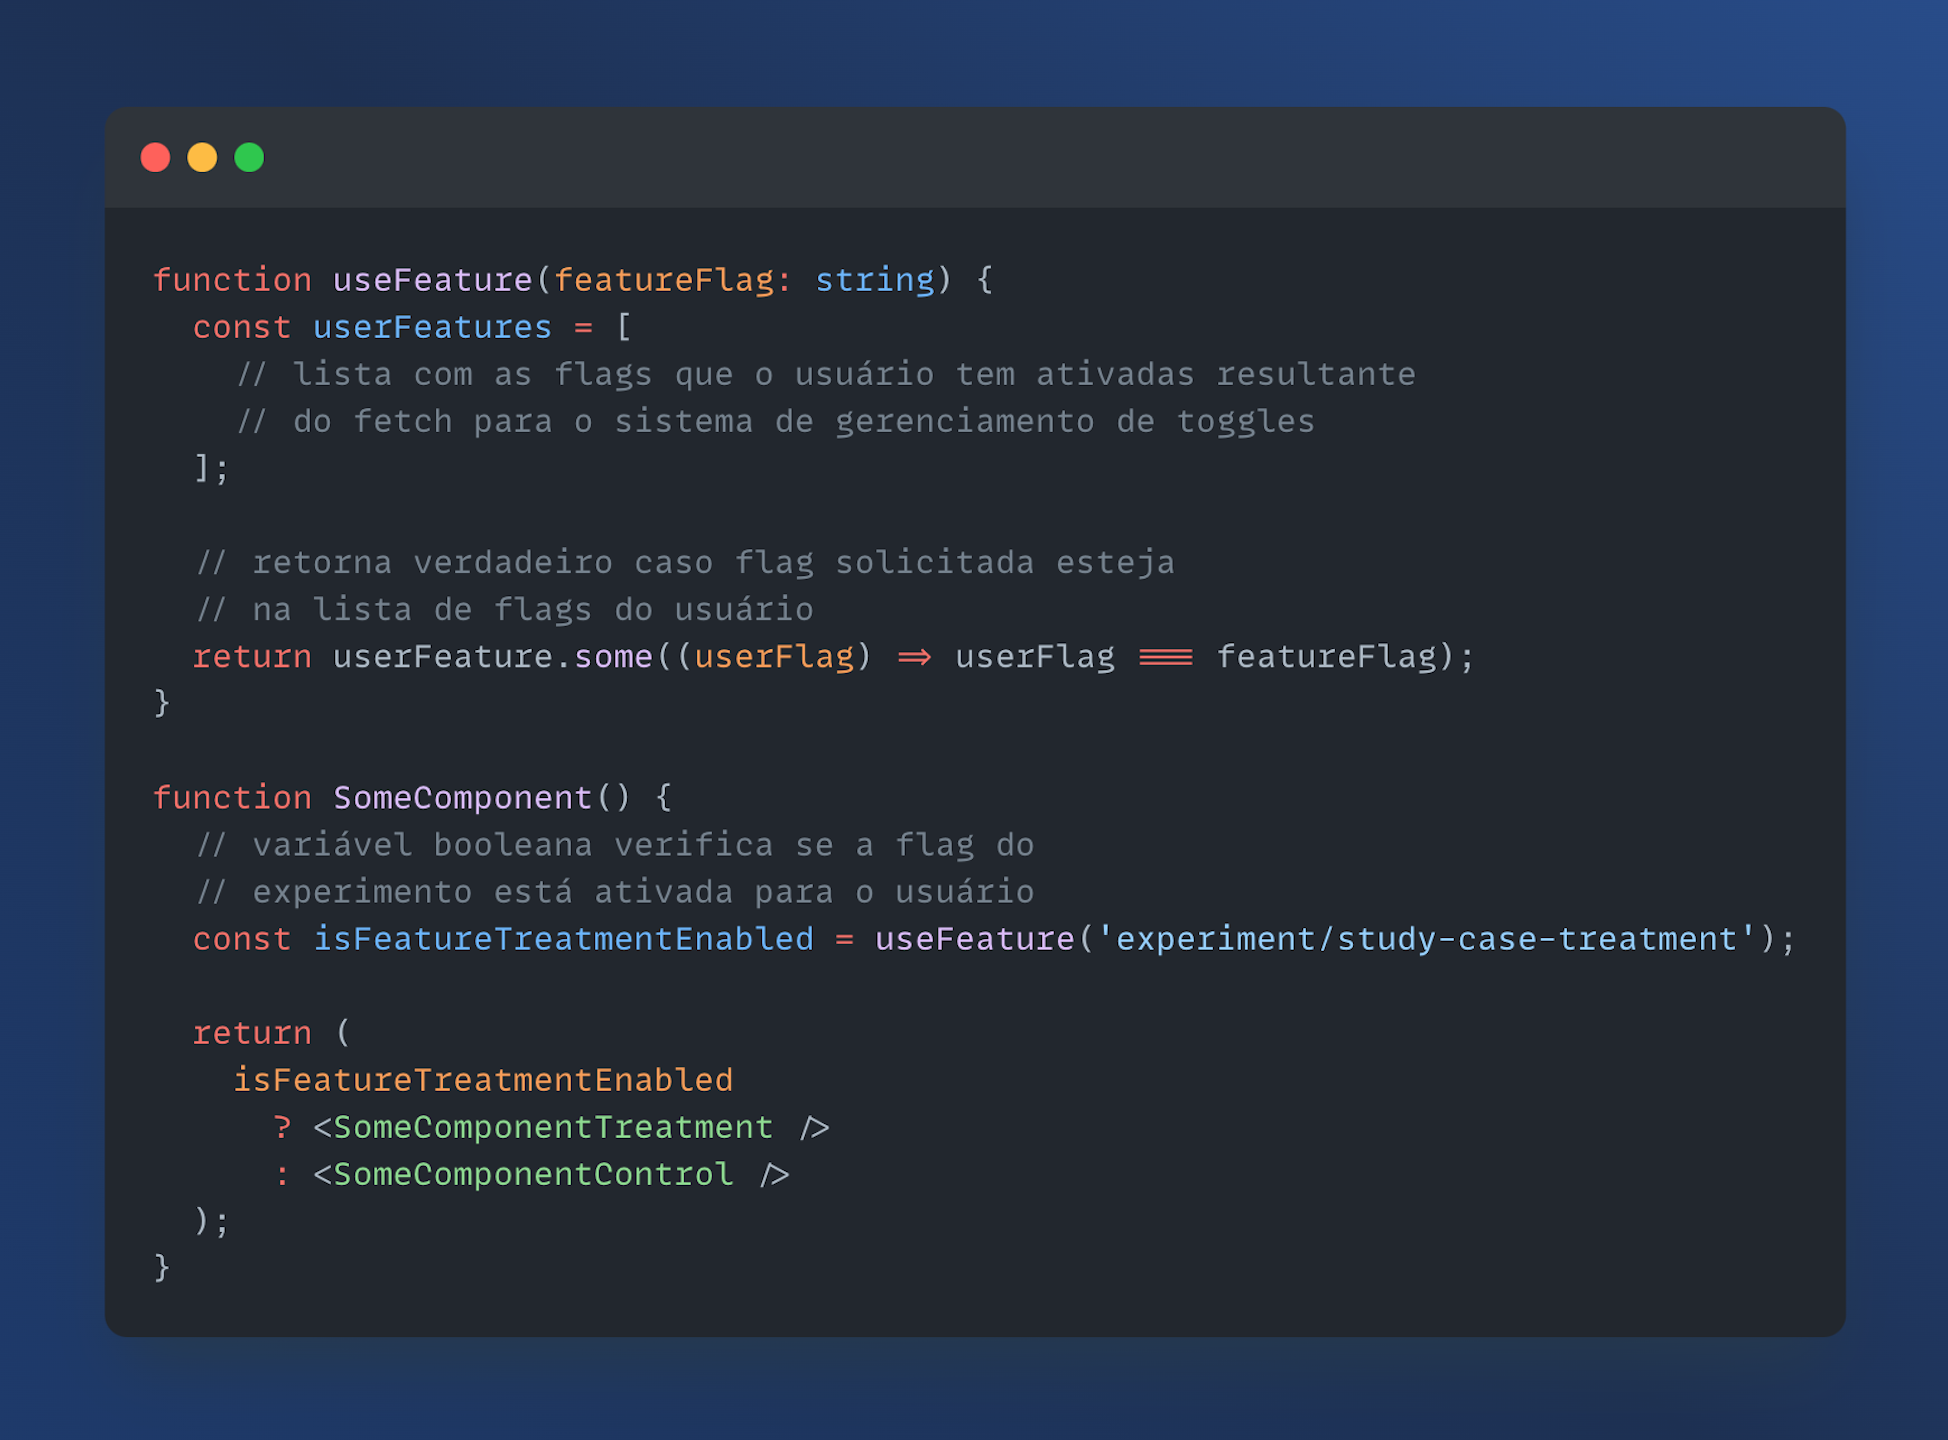
\includegraphics[width=1\linewidth]{figuras/toggle.png}
    \begin{center}
        \text{Fonte: Autor}
    \end{center}
    \label{fig:toggle}
\end{figure}